\seclab{Method and Theory}{methodandtheory}


\subsection{Creation of experimental setup}
In order to produce a model to determine age based on facial images, it is necessary to gather some training data. The training data would in the case of this report be a set of human responses, an estimate of age, to a collection of stimuli, in the form of a series of human faces. However, before such an experiment can be set up, it is necessary to develop a nice collection of human faces in various age groups to present as stimulus. In order to get a nice spread of age groups we chose to use the IMDB-WIKI data set \cite{IMDB15,IMDB16}. According to the providers, the IMDB-WIKI data set is the largest publicly available data set of face images with gender and age labels for the training of machine learning models (ML). The data set contains 460,723 face images of 20,284 celebrities from IMDB as well as 62,328 images from Wikipedia. For the purpose of this project we chose only to focus on the images from IMDB as these seemed to be of greater quality and had a less skewed distribution of ages as evidenced in \figref{age_dist}.

\begin{figure}[ht]
    \centering
    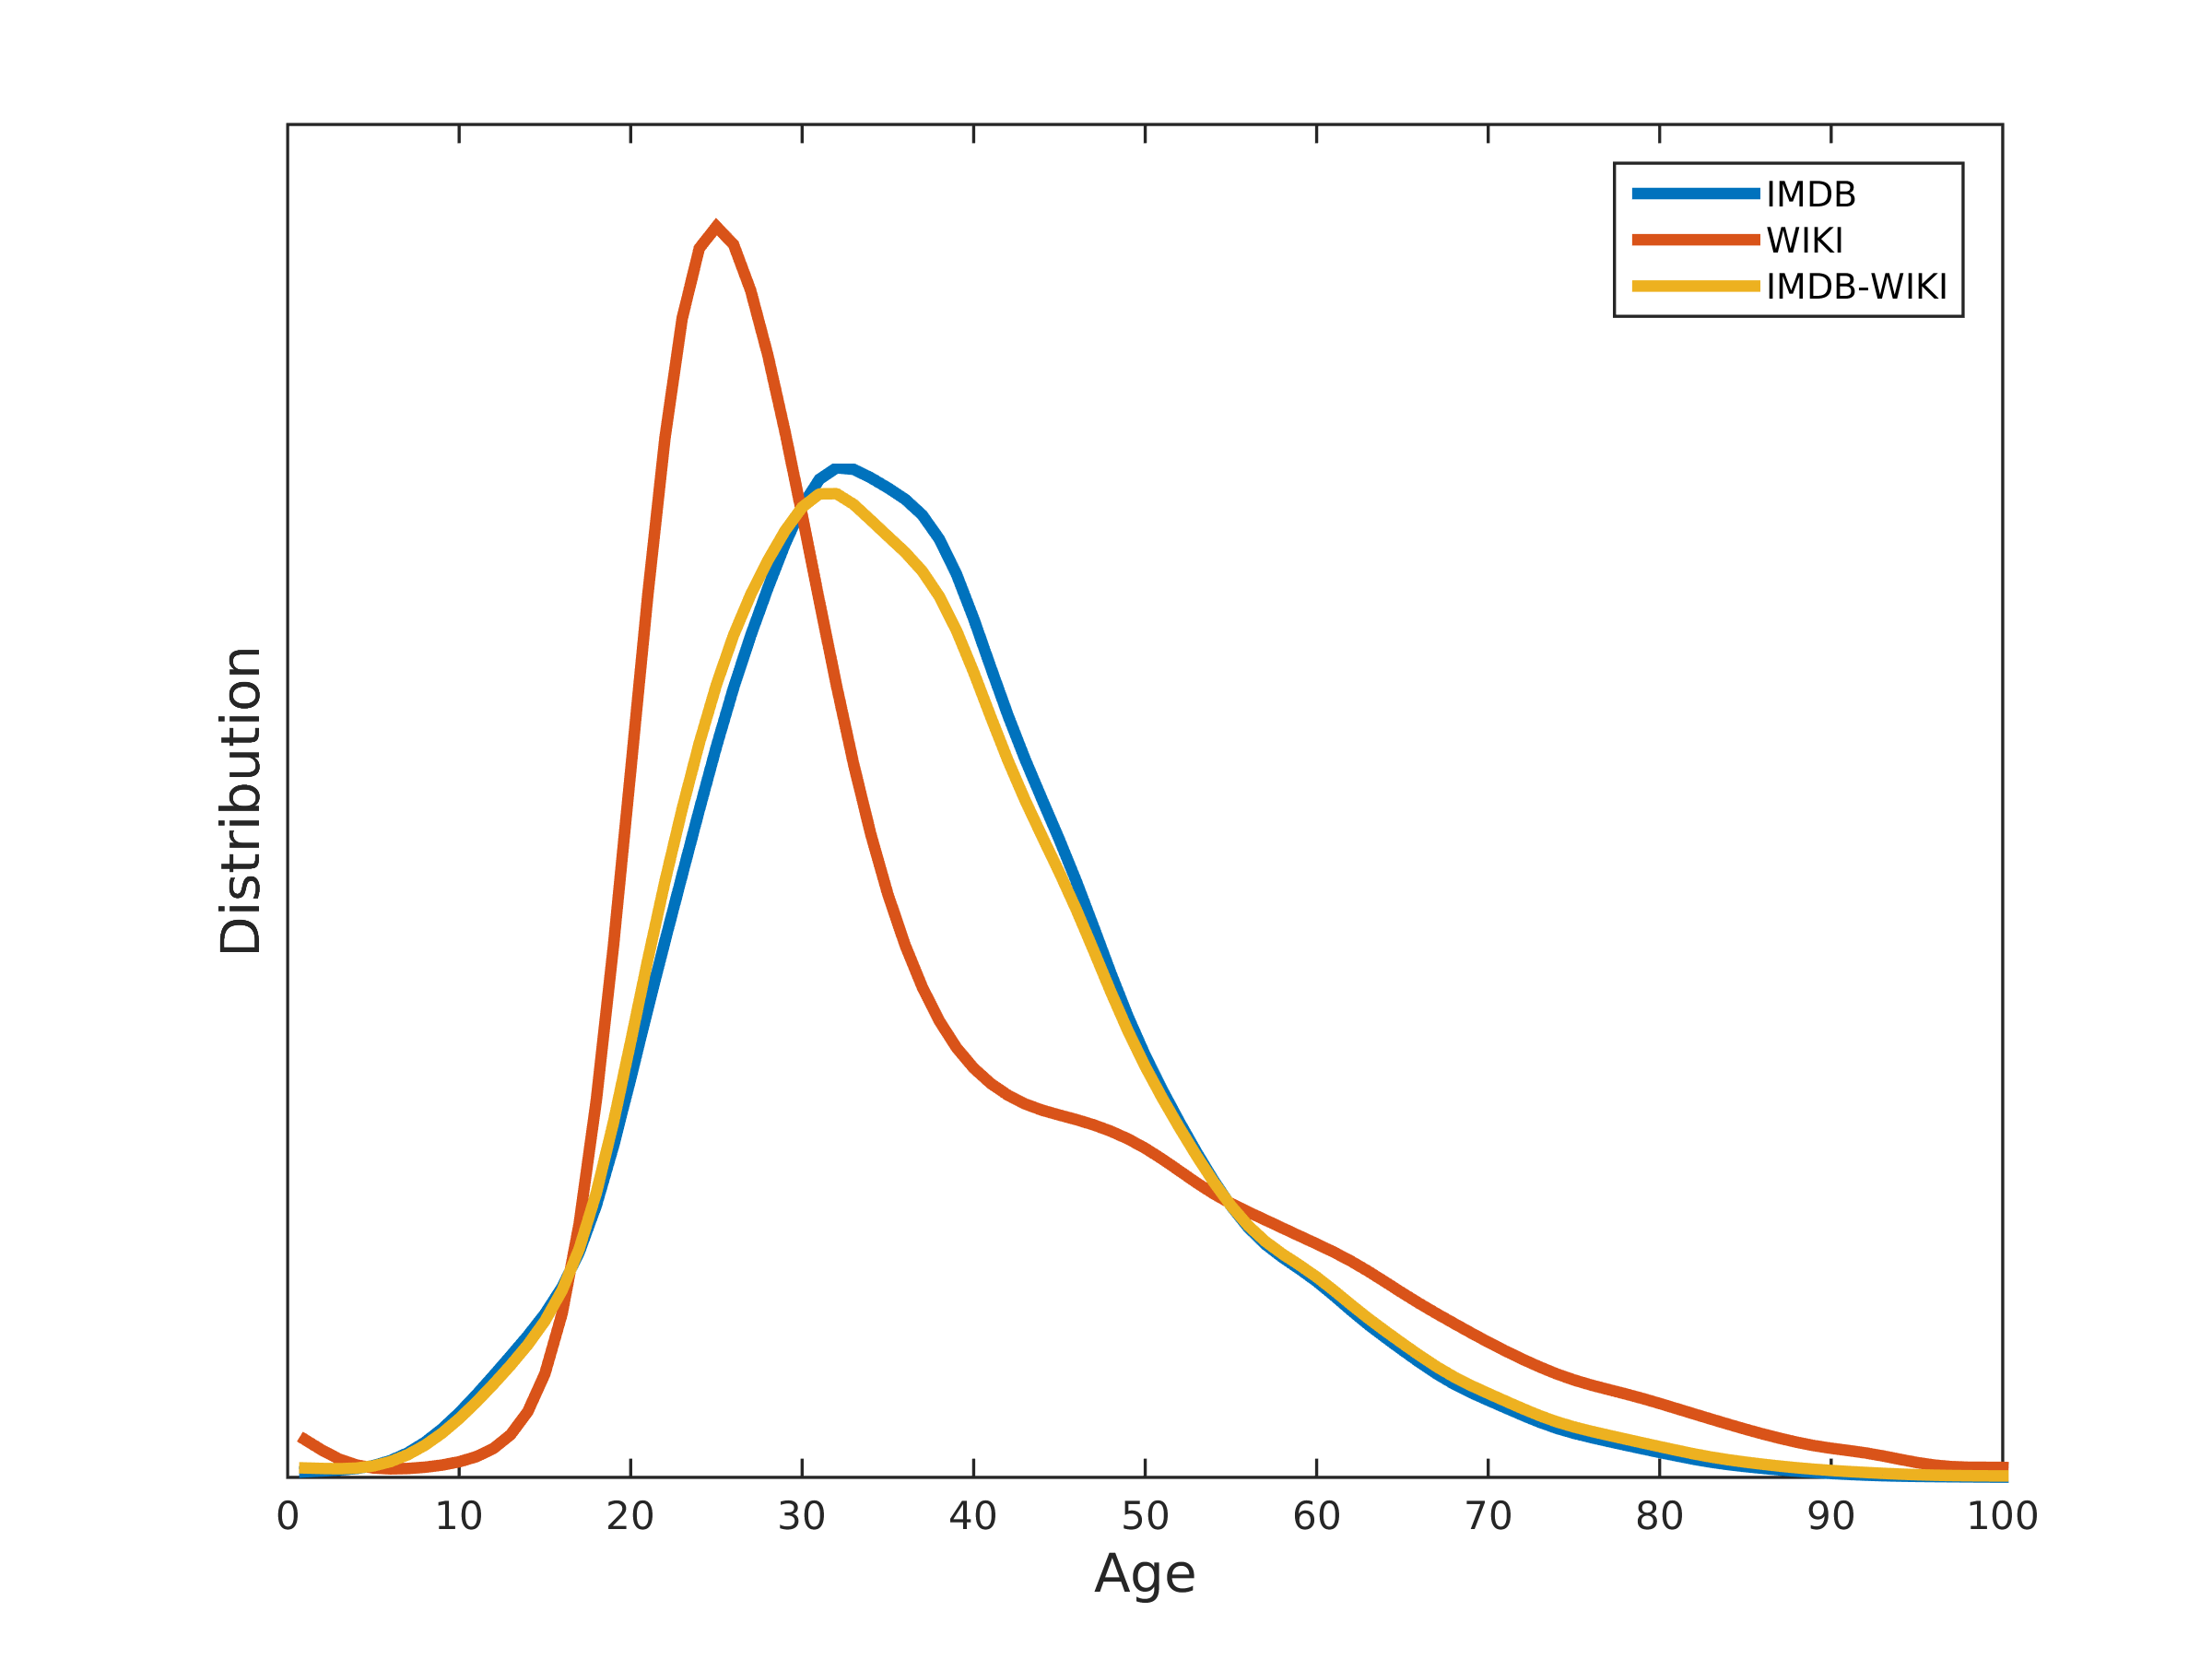
\includegraphics[width = 0.9\linewidth]{fig/age_dist.png}
    \caption{Distribution of ages in the IMDB-WIKI data set}
    \label{fig:age_dist}
\end{figure}

Having found a large data set with a considerable span in age and gender, the next step was to standardize the images in such a way that they could be compared. This was necessary as to ensure that the same physical features of the human faces would appear in roughly the same pixel patches for each image such that we would have a well-defined average face for both men and women. Another important point was to ensure that we got a relatively even distribution of ages as well as genders. To do this, we loaded the images into MATLAB where-after we wrote a script ensuring that we could manually approve each image before saving it to the final data set to be used for our cognitive experiment. Essentially the script randomly selects one of the pictures from the set with a dimensionality of at least 300 by 300 pixels, and crops it using MATLAB's CascadeObjectDetector. The CascadeObjectDetector is a system object using the Viola-Jones algorithm to detect people’s faces, noses, eyes, mouths, or upper body \cite{viola-jones}. Thus we simply cropped the input image to the pixels in which a face was recognized and thereafter re-sized it to a 500$\times$500 pixel image. The image was then displayed to the user together with the given labels associated for validation. This was a necessity as some of the images contained more than one person and thus the given label might have been associated with a person different from the one caught by the CascadeObjectDetector. If the image got manually approved, the image would be transformed into grayscale and stored in matrix form to the appropriate predefined age group bucket (a tensor of rank 3) based on the image's age label. The reason for grayscaling the image was not only to reduce the dimensionality of the images, but also to ensure that the conclusions gotten from data processing would be solely based on facial features without the noise generated by colour. A total of 5 age group buckets, linearly splitting an age span from 10 to 80 years, were predefined for both males and females, each of which would ultimately contain 50 unique images. 

The result would thus be a data set consisting of 250 images of relatively even age distribution for each gender. The reason for splitting the data set by gender, lies in the inherent difference between male and female faces, and thereby the features important for age. As to ensure that different pictures of the same actor/actress would be excluded from the final data set, the celebrity id (a unique id to distinguish actors/actresses in the original data set) was stored to a vector and used as a filter for the input images.\footnote{That being said, it could have been tremendous to have a data set consisting of 250 pictures of the one and only Samuel L. Jackson (what a \textbf{man!})}

Having generated a set consisting of 250 faces, distributed evenly in age, for both males and females, we continued preparing an experiment to test how given subjects perceive age. The experiment was conducted in the following manner. Each subject was asked to look through the 250 images for each gender, typing in the age that first came to mind when viewing the image. After a couple of attempts it was realized that the constructed data set was not completely ideal in the sense that it contained well known actors/actresses, implying that the subjects seemed to have a bias, i.e. an idea of the age of the shown image. This effect was however mitigated to some extent by actively asking the subjects to judge the age solely on the facial features presented, but also naturally by the fact that some of the images were from old movies implying that the knowledge of current age became useless. In total we managed to gather the input of 3 individuals for the male data set and the input of 5 individuals for the female data set.

As to ensure that no outliers would be included in the data for analysis, a filter was implemented checking the difference in the inputted ages for the male and female data sets. If, for a given image, the absolute difference in age was over 20 years, the image was disregarded from the set. This excluded a total of 2 images for the males and 5 images for the females. In \figref{avgface} the average male and female face composed of the 248 and 245 images respectively can be seen. This confirms that the images chosen for the experiments indeed are comparable and centered, as we get a relatively clear depiction of a human face. 

\begin{figure}[ht]
    \centering
    \begin{minipage}{0.49\textwidth}
    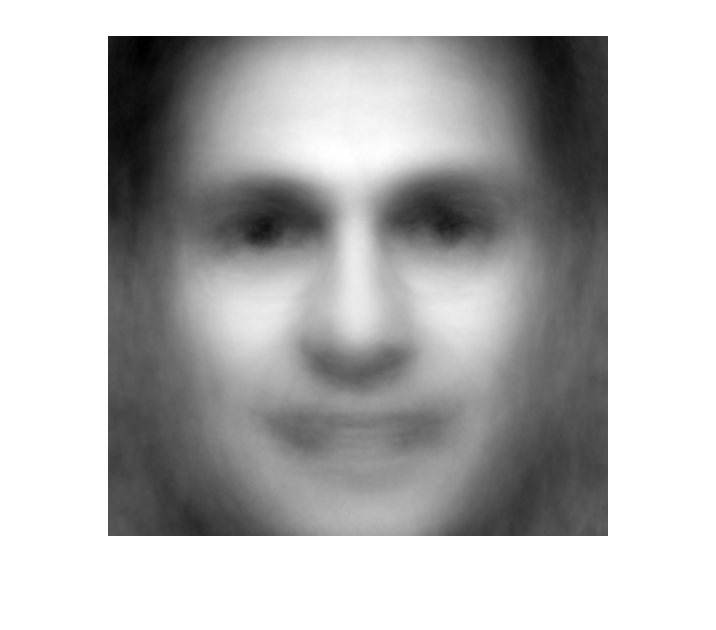
\includegraphics[width=1\textwidth]{fig/henrikbruus.png}
    \end{minipage}
    \begin{minipage}{0.49\textwidth}
    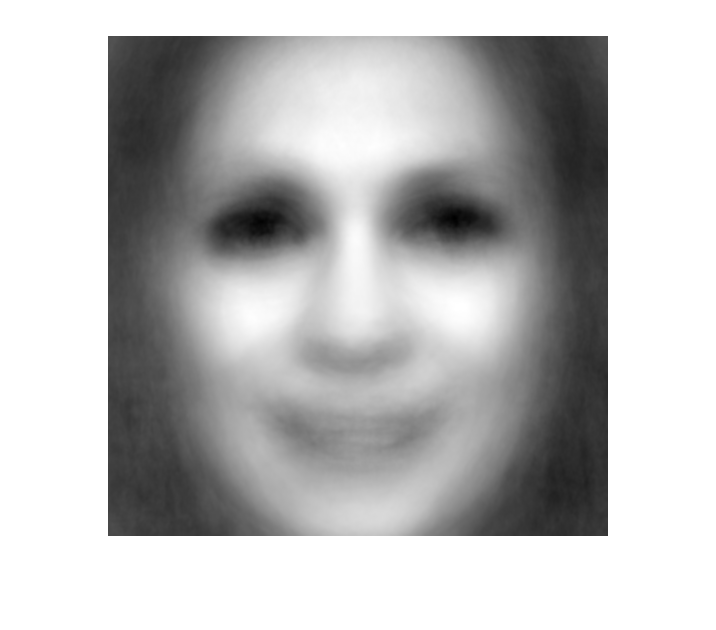
\includegraphics[width=1\textwidth]{fig/henrikbruuskone.png}
    \end{minipage}
    \caption{Left: The average face composed of the 248 male images. Right: The average face composed of the 245 female images.}
    \label{fig:avgface}
\end{figure}

\subsection{Method used for modelling}
Due to the humongous dimensionality of the rank 3 tensors created for image storage as part of the experimental setup, the amount of processing power needed to do real modelling of the data was extensive and hence dimensionality reduction was appropriate, or rather, a necessity. To be more exact, the dimensionality of each rank 3 tensor is $500 \mathrm{(height)} \times 500 \mathrm{(width)} \times 250 \text{(number of gender specific pictures)}= 6.25 \times 10^{7}$. There exists several methods for dimensionality reduction with the ones touched upon in the course being Principal Component Analysis (PCA) and Independent Component Analysis (ICA). Other methods include auto-encoders (deep artificial neural networks) which can be very efficient, but possess the disadvantage that we would miss the interpretable cognitive properties of our sought model. This is due to the face that auto-encoders make highly non-linear mappings that are hard to track.

\subsubsection{Principal Component Analysis (PCA)}
As alluded to in the previous section, a reduction in dimensions will be necessary if any computations and transformations are to be feasible. However, there is another stronger argument for performing a PCA rooted in the modest proposal, that information is represented in an efficient way in the human brain. To elaborate, this rests on the belief that although the human brain receives many signals from its environment, it will not make a one-to-one mapping of these signals to produce a representation of the external environment. Instead, in the essence of being efficient, it will attempt to decorrelate the signals received in the receptors to a representation sufficient for survival \cite{PCA1}. The human brain already consumes 20\% of a humans total energy consumption, spending more energy in an attempt to for example render the single hair strand of a tiger would simply not make any sense, as you could use a significantly lower amount of effort and energy in simply identifying the threat of a tiger by the orange and black stripes \footnote{This is not to say that you should run for your life if you see orange and black stripes as you are strolling through the city of Copenhagen, you should however strongly consider it if you're in an Indian jungle.}. In the light of this discussion, one could claim that PCA functions in much the same way. Instead of gathering all the information from the image in question, most of the vital information for cognitive tasks, such as determining the age of a person on the basis of his or her facial features, can be extracted by considering a significantly lower dimensionality. 

On a practical level, before performing the PCA, it was necessary to re-scale the images from 500$\times$500 pixels to 100$\times$100 pixels to make any further transformations feasible. Although this may sound like a serious reduction of information, we feel it safe to assume that the features important for age-determination would still present themselves in the dimension reduced images. If time allowed for a rerun of the experiment, we would have presented the 100 by 100 pixel images to ensure that no information be lost. We then flattened each of the images to a $100 \mathrm{(height)} \times 100 \mathrm{(width)} = 10,000$ dimensional vector, and placed them as consecutive rows in a $N$ by 10,000 matrix for each gender, where $N$ is the total number of images for the given gender. The matrix was then normalized by subtracting the mean from each of the observations and dividing by the standard deviation pixel-wise. PCA was then evaluated on the resulting normalized matrix. The results can be seen in \figref{PCA} where the first 16 eigenfaces have been displayed for both the males and females. An eigenface is in it's essence a principal component that has been restructured to a, in this case, 100 by 100 matrix as to resemble an image. One can therefore think of eigenfaces as being the building blocks of any facial image by the weighted sum of the eigenfaces. For instance a face $F$ could be evaluated as $F = 23\%E_1 + 50\%E_2 - 17\%E_3 + ... + 1\%E_n$, where $E_i$ represents the $i$'th eigenface, $n$ denotes the number of eigenfaces considered for the reconstruction and the percentages are the weights associated to each eigenface (and can be negative). We will talk more about reconstruction of images later.

\begin{figure}[ht!]
    \centering
    \begin{minipage}{0.49\textwidth}
    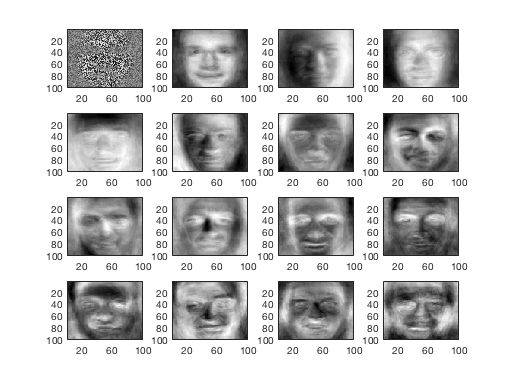
\includegraphics[width=1\linewidth]{fig/M_PCA.png}
    \end{minipage}
    \begin{minipage}{0.49\textwidth}
    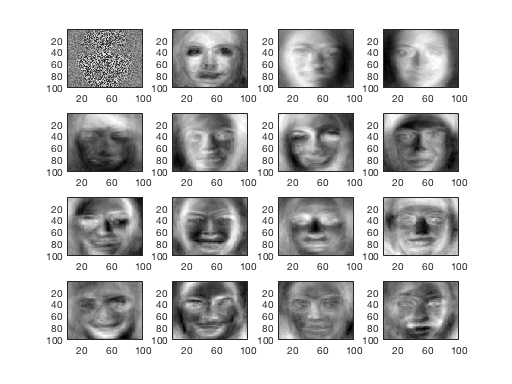
\includegraphics[width=1\linewidth]{fig/F_PCA.png}
    \end{minipage}
    \caption{Left: The 16 eigenfaces with highest variance for the males sorted by descending variance. Right: The 16 eigenfaces with highest variance for the females sorted by descending variance.}
    \label{fig:PCA}
\end{figure}

As evident from \figref{PCA}, the first eigenface for both males and females looks like random noise, which makes a lot of sense, since we have normalized the data. The eigenface with the second highest variance seems to be a generic male and female face from which most of the gender specific features can be extracted. Another point to make is that, for both men and women, the next couple of eigenfaces seem to be related to a lighting of the face from the sides and from top and bottom. It is also worth mentioning that some of the less important eigenfaces seem to be concerned with facial symmetry, facial hair and sizes of noses, eyes and mouths. In order to find the appropriate number of eigenfaces to consider for further analysis, we will set a threshold for the variance explained by the eigenfaces and choose the minimum number of eigenfaces required to obtain the threshold. 

\begin{figure}[ht!]
    \centering
    \begin{minipage}{0.19\textwidth}
    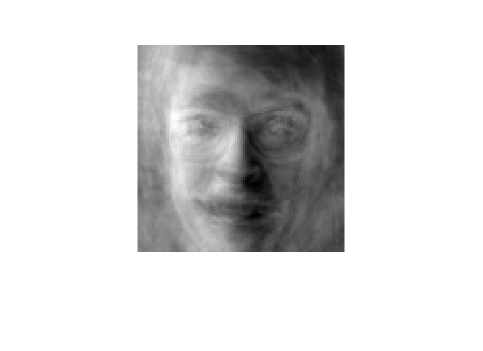
\includegraphics[width = 1\textwidth]{fig/petyr_80.png}
    \end{minipage}
     \begin{minipage}{0.19\textwidth}
    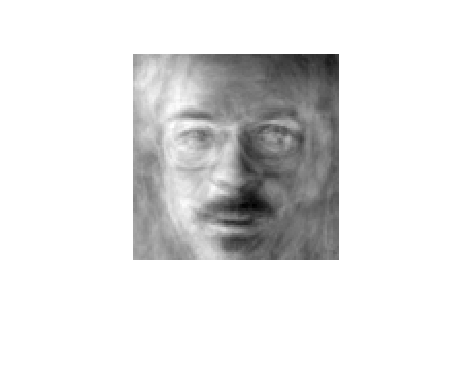
\includegraphics[width = 1\textwidth]{fig/petyr_90.png}
    \end{minipage}
     \begin{minipage}{0.19\textwidth}
    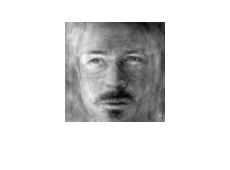
\includegraphics[width = 1\textwidth]{fig/petyr_95.png}
    \end{minipage}
     \begin{minipage}{0.19\textwidth}
    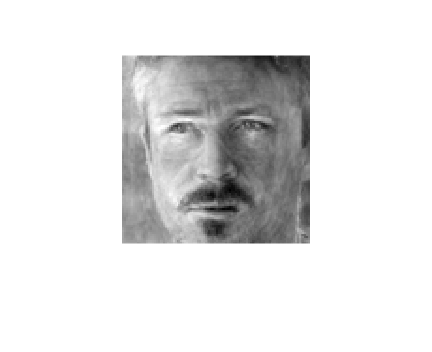
\includegraphics[width = 1\textwidth]{fig/petyr_99.png}
    \end{minipage}
     \begin{minipage}{0.19\textwidth}
    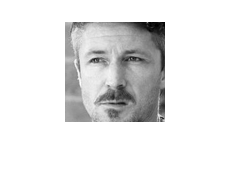
\includegraphics[width = 1\textwidth]{fig/petyr_100.png}
    \end{minipage}
    \caption{Reconstruction of a male face using the number of eigenfaces capable of explaining 80\%, 90\%, 95\%, 99\% and 100\% of the variance respectively.}
    \label{fig:petyr}
\end{figure}

In \figref{petyr}, we see the same male face reconstructed using an increasing number of eigenfaces. Specifically they have been created using variance thresholds of 80\%, 90\%, 95\%, 99\% and 100\% using a total of 27, 64, 110, 195 and 248 respectively (since the given image depicts a person of the male gender). As evident, the difference in the quality of the reconstruction is significantly reduced as the total number of eigenfaces is increased. For the remainder of the report, we will use the 90\% variance threshold for the principal components, corresponding to a total of 64 eigenfaces to consider for both blokes and sheilas.

\subsection{The Multi-Linear Regression}
Ideally, we would like to create an interpretable supervised model which accurately predicts how our subjects perceive age. That would be a model generalizing well which can be identified with a model having a small test error in \figref{model_complexity}. To train a supervised learning model such that we can obtain a small error, it is important to consider the complexity of the model one should make. For this purpose, we could fairly easily be able to create an artificial neural network (ANN) which could create some non-linear mappings resulting in a small error. However, it would take the interpretability out of the model since the interpretability of ANNs is very limited. Hence, we decided to create a multi-linear regression model using the Least Absolute Shrinkage and Selection Operator (Lasso) as we would like the model to be interpretable. The Lasso is used for regularization and dimensionality reduction such that only the most important eigenfaces ends up having non-zero weights. To elaborate further on the choice of regularization, i.e. the \Lnorm{1} (Lasso), we will first need to introduce the ordinary least squares regression and the objective function that we are trying to minimize.  \\
From the executed experiments done by our subjects, we created two data sets for modelling (one for each gender) with $N_{\mathrm{male}} = 248$ male observations, and $N_{\mathrm{female}}=245$ female observations. Lets denote an observation by a feature vector $\vec{x}_i$ and a target $y_i$ which is the perceived age of a given face. The feature vector $\xxx_i$ is a $M$-dimensional vector consisting of the projection-weights of a given photo onto the PCs found by PCA to achieve a given percentage of the total variance in the original picture for men and women respectively (in this case 90\%). The target $y_i$ for each image is taken to be the mean age perceived by our subjects. All data pairs $\curlyb{\xxx_i,y_i}_{i=1}^N$ are then gathered into data sets $\qty(\XXX_{\male},\yyy_{\male})$ and $\qty(\XXX_{\female},\yyy_{\female})$ separately.\footnote{With $\XXX_{\male}$ having dimension $N_{\male} \times M$ and $\yyy$ having dimension $N_{\male}$. The only difference to the dimension of the female set being that $N_{\male} \neq N_{\female}$.} \\ 
Having assumed that we can establish a linear relationship between a feature vector $\xxx_i$ and its corresponding target $y_i$, i.e., we can write a predicted target on the form $y_i = f\qty(\xxx_i,\vec{w})= \xxx_i^{\top} \vec{w}$ (due to the fact that the data is centered from PCA), where the optimal weights $\vec{w}^{\ast}$ are found by minimizing the objective function in the ordinary least squares regression (OLS) \cite{allhailkingMorten},
\begin{equation}\label{eq:RSS}
    \www^{\ast} = \argmin_{\www}\curlyb{ \dfrac{1}{N} \sum_{i=1}^N \qty(y_i - f\qty(\xxx_i,\www))^2 } = \argmin_{\www}\curlyb{\dfrac{1}{N} \sum_{i=1}^N \qty(y_i - \xxx_i^{\top} \www)^2 }
\end{equation}

\begin{figure}[t]
    \centering
    \begin{tikzpicture}[scale=3]
        \draw[] (0,0) rectangle (3,2);
        \draw[softblue, thick] (0.2,1.5) .. controls (0.9,0.65) and (2,1) .. (2.5,1.2);
        \draw[black, thick] (0.2,1.4) .. controls (0.9,0.5) and (2,0.4) .. (2.5,0.2);
        \draw[->, dotted, thick] (0.7,1.55)--(0.2,1.55);
        \draw[->, dotted, thick] (2.2,1.55)--(2.7,1.55);
        \node[anchor=south] at (2,1.1) {Test Error};
        \node[anchor=south] at (1.7,0.15) {Training Error};
        \node[anchor=west] at (2.1,1.9) {Low Bias};
        \node[anchor=west] at (2.1,1.7) {High Variance};
        \node[anchor=west] at (0.1,1.9) {High Bias};
        \node[anchor=west] at (0.1,1.7) {Low Variance};
        \node[anchor=west] at (0,-0.1) {Low};
        \node[anchor=east] at (3,-0.1) {High};
        \node[anchor=south, rotate= 90] at (-0.1,1) {Prediction error};
        \node[anchor=north] at (1.5,-0.1) {Model Complexity};
    \end{tikzpicture}
    \caption[Model complexity vs prediction error]{Illustration of the Bias-Variance trade-off in model selection.}
    \label{fig:model_complexity}
\end{figure}


\subsubsection{The Least Absolute Shrinkage and Selection Operator (Lasso) and the Ridge regression}
As the objective function in the OLS regression does not take into account that the weights might have a prior probability distribution, it does not really match our purpose since we want to find a sparse solution, i.e., a low-dimensional feature vector containing the important eigenfaces for predicting how our subjects perceive facial age. Ideally, the weight distribution would look more like a Laplacian distribution and thus we chose to regularize with Lasso. We also considered the Ridge regression which regularizes with the \Lnorm{2} and assumes that the prior distribution of the weights follow a normal distribution. But applying a Ridge regression would not allow for as sparse solutions as using a Lasso regularization. To elaborate further, looking at \figref{lassovsridge} we see the contours which are the weights of the OLS solution. The solution to minimizing the objective functions for the Lasso- and Ridge regressions respectively are seen in the figure as the points where the contours hit the constraint regions, i.e, touches the \Lnorm{1} (Lasso) and \Lnorm{2} (Ridge) regions.\footnote{This figure is produced for illustrative purposes and the concept can be extended to higher dimensions.} Hence this illustrates why weights rarely go all the way to zero for the Ridge regression since there are no edges, whereas the Lasso solution allows for sparse solutions which is also evident from the geometric representation. After having argued why we went for a Lasso regularization it seems appropriate to introduce the objective function for such a regression type, 
\begin{equation}\label{eq:Lasso}
    \www^{\ast} = \argmin_{\www}\curlyb{ \dfrac{1}{N} \sum_{i=1}^N \qty(y_i - f\qty(\xxx_i,\www))^2 + \lambda \norm{\www}_1}
\end{equation}
where $\lambda$ is called the regularization strength \cite{Tibshirani94regressionshrinkage}. From \eqref{Lasso} it is evident that if the regularization strength $\lambda$ is increased, the norm of the weights will have to decrease. Another purpose for regularization, is that it allows for the tuning of model complexity to hit the right amount of bias and variance as shown in \figref{model_complexity}. Additionally to using Lasso for model selection and performance evaluation we used Cross-validation (CV), which is a technique which can optimize hyper-parameters (model selection) and give the best possible estimation of the true test error through an idealized quantity called the generalization error \cite{allhailkingMorten}.\footnote{Further elaboration on this can be found in \appref{appendix}}

\begin{figure}[t]
    \centering
    %First pictures
   
    \begin{subfigure}[b]{0.45\textwidth}
        \begin{tikzpicture}
            \begin{axis}[no markers,xlabel=$\hat{w}_1$, 
                ylabel=$\hat{w}_2$,
                ticks=none,
                axis x line=center,
                axis y line=center,
                ymin=-1.1,
                xmin=-1.1,
                xmax=2,
                ymax=3,
                axis equal]
                \addplot+[fill=softgrey, color=softgrey, opacity=0.5] coordinates
                {(-1,0) (0,1) (1,0) (0,-1)}--cycle;
                \draw[red] (1,2) ellipse [x radius=0.4, y radius=0.2, rotate=45];
                \draw[red] (1,2) ellipse [x radius=0.6, y radius=0.3, rotate=45];
                \draw[red] (1,2) ellipse [x radius=1, y radius=0.5, rotate=45];
                \draw[red] (1,2) ellipse [x radius=1.4, y radius=0.7, rotate=45];
                \node[] at (1,2) {$\hat{w}$};
            \end{axis}
            %
        \end{tikzpicture}
    \end{subfigure}
    \quad
    %Second picture
    \begin{subfigure}[b]{0.45\textwidth}
        \begin{tikzpicture}
            \begin{axis}[no markers,xlabel=$\hat{w}_1$, 
                ylabel=$\hat{w}_2$,
                ticks=none,
                axis x line=center,
                axis y line=center,
                ymin=-1.1,
                xmin=-1.1,
                xmax=2,
                ymax=3,
                axis equal]
                \filldraw[draw=softgrey, fill=softgrey, opacity=0.5] (0,0) circle (1);
                \draw[red] (1,2) ellipse [x radius=0.4, y radius=0.2, rotate=45];
                \draw[red] (1,2) ellipse [x radius=0.6, y radius=0.3, rotate=45];
                \draw[red] (1,2) ellipse [x radius=1, y radius=0.5, rotate=45];
                \draw[red] (1,2) ellipse [x radius=1.3, y radius=0.65, rotate=45];
                \node[] at (1,2) {$\hat{w}$};
            \end{axis}
        \end{tikzpicture}
    \end{subfigure}
    
    \caption[Lasso versus Ridge Shrinkage]{Geometric representation of the solutions to the Lasso (Left pane) and the Ridge (Right pane) respectively.}
    \label{fig:lassovsridge}
\end{figure}

%%%%%%%%%%%%%%%%%%%%%%%%%%%%%%%%%%%%

